
\begin{lead}

 ディジタル信号処理の重要な応用分野として画像処理がある.本章では,その基礎に関しての説明を行う.前章で説明したディジタルフィルタに関する記述は,この画像処理を理解する上で重要なものであり,その内容を理解しているという前提のもとで,本章では,ディジタル画像の表現と画像の周波数解析について説明する.

\end{lead}

%\vfill

%\begin{koumoku}
%アナログフィルタ\\
%ディジタルフィルタ\\
%IIRフィルタ\\
%FIRフィルタ\\
%\end{koumoku}

%\clearpage

\chapter{\index{でぃじたるがぞう@ディジタル画像}ディジタル画像の表現}

\label{chapter:image}

\section{画像信号の表現}

画像には種々の種類があり,その表現や処理方法が異なる.

\subsection{表示条件による分類}

画像を表示条件で分類すると,以下のように記述できる.

\begin{itemize}
\item 色や明暗に関する分類\\
明暗の情報だけを持つ画像を白黒画像または\index{のうたんがぞう@濃淡画像}濃淡画像という,また,色の情報を持つ画像は\index{からーがぞう@カラー画像}カラー画像という.
\item 時間に対する変化での分類\\
時間的に変化しない画像を\index{せいしがぞう@静止画像}静止画像といい,時間的に変化する画像を\index{どうがぞう@動画像}動画像という.
\item 画像の階調の大小に関する分類\\
白と黒の2階調を持つ画像を\index{2ちがぞう@2値画像}2値画像,256階調以上の自然な連続した階調の画像を\index{しぜんかいちょうがぞう@自然階調画像}自然階調画像,それらの中間の階調を持つ画像を\index{ちゅうかんかいちょうがぞう@中間階調画像}中間階調画像という.
\end{itemize}

\subsection{処理手法による画像処理の分類}

画像処理を処理手法で分類すると,以下のように記述できる.

\begin{itemize}
\item \index{がぞうあっしゅく@画像圧縮}画像圧縮\\
画像情報を表すためのデータ量は,音声などと比べると通常膨大となる.一般的に画像情報には偏りがあることから,これを利用してデータ量を削減する技術が画像圧縮である.画像通信やメモリへの記憶の際に不可欠な技術である.
\item \index{がしつかいぜん@画質改善}画質改善\\
画質改善とは,ひずみや雑音によりダメージを受けた画像の画質を改善する技術である.
\item \index{がぞうかいせき@画像解析}画像解析\\
画像解析とは,与えられた画像の構造を分析して,その特徴を抽出して処理を行う技術である.これはしばしば,画像の認識・理解とも呼ばれる.
\end{itemize}

\subsection{ディジタル画像信号}

ここでは,\index{でぃじたるがぞうしんごう@ディジタル画像信号}ディジタル画像信号の表現法を説明する.

\subsubsection{信号の次元}

音声信号は1次元信号,静止画像は2次元信号,動画像は3次元信号といわれる.

まず,1次元信号である音声信号$f(t)$について,図\ref{fig:zu-07-2}(a)のように図的に表現する.これは,ある時刻$t_0$を規定すると対応値$f(t_0)$が一意的に決まることを意味する.このことから,その値が1変数関数として表現できる信号を1次元信号という.

静止画像のような2次元信号は,場所$x,y$の関数$f(x,y)$として表される.ここで関数$f(x,y)$のとる値は輝度値に相当するものが用いられる.カラー画像の場合であれば,RGB (Red, Green, Blue) やCMYK (Cyan, Magenta, Yellow, Key plate)の各成分が用いられる.


\begin{figure}[H]
\begin{center}
\begin{minipage}{.35\textwidth}
\begin{center}
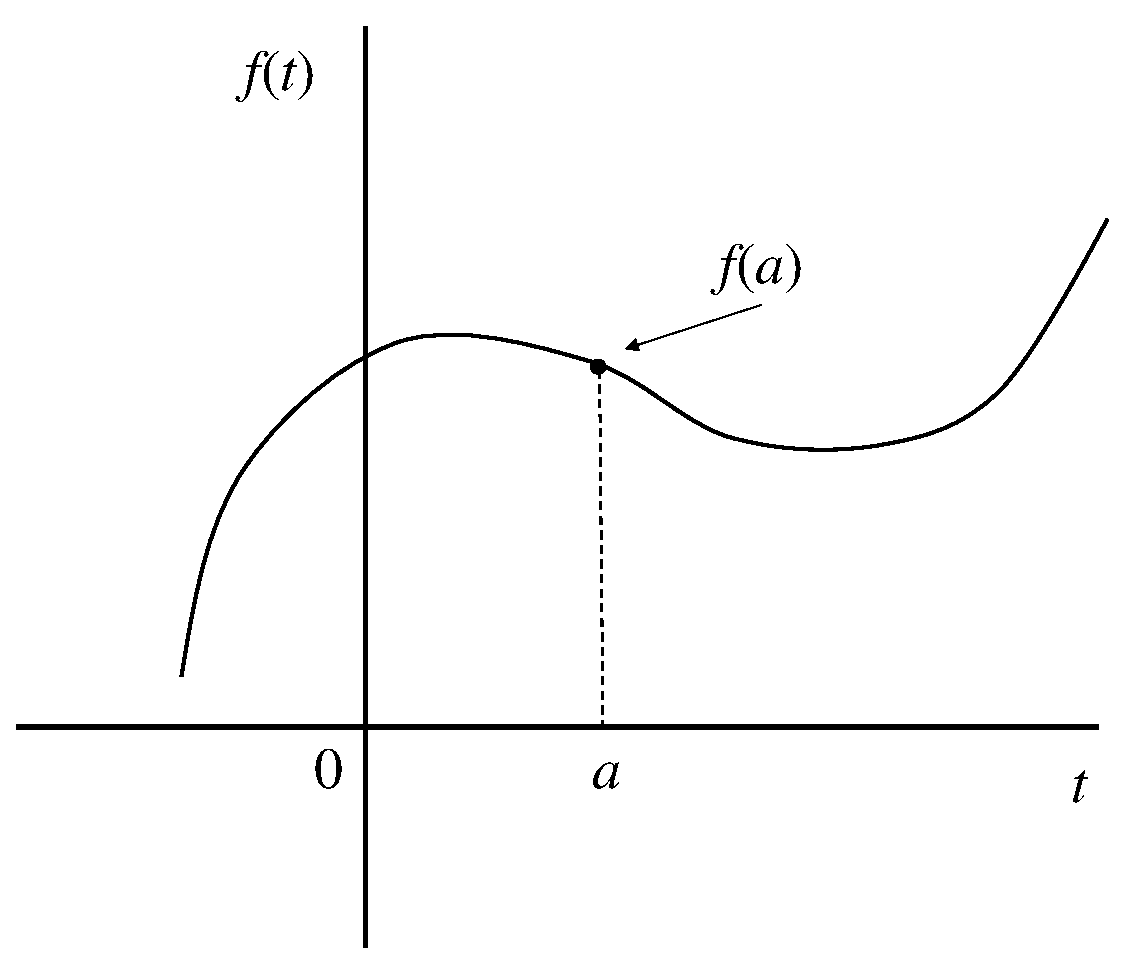
\includegraphics[width=.98\textwidth]{fig/zu-7-2-a.eps}

(a) 1次元信号
\end{center}
\end{minipage}
\begin{minipage}{.35\textwidth}
\begin{center}
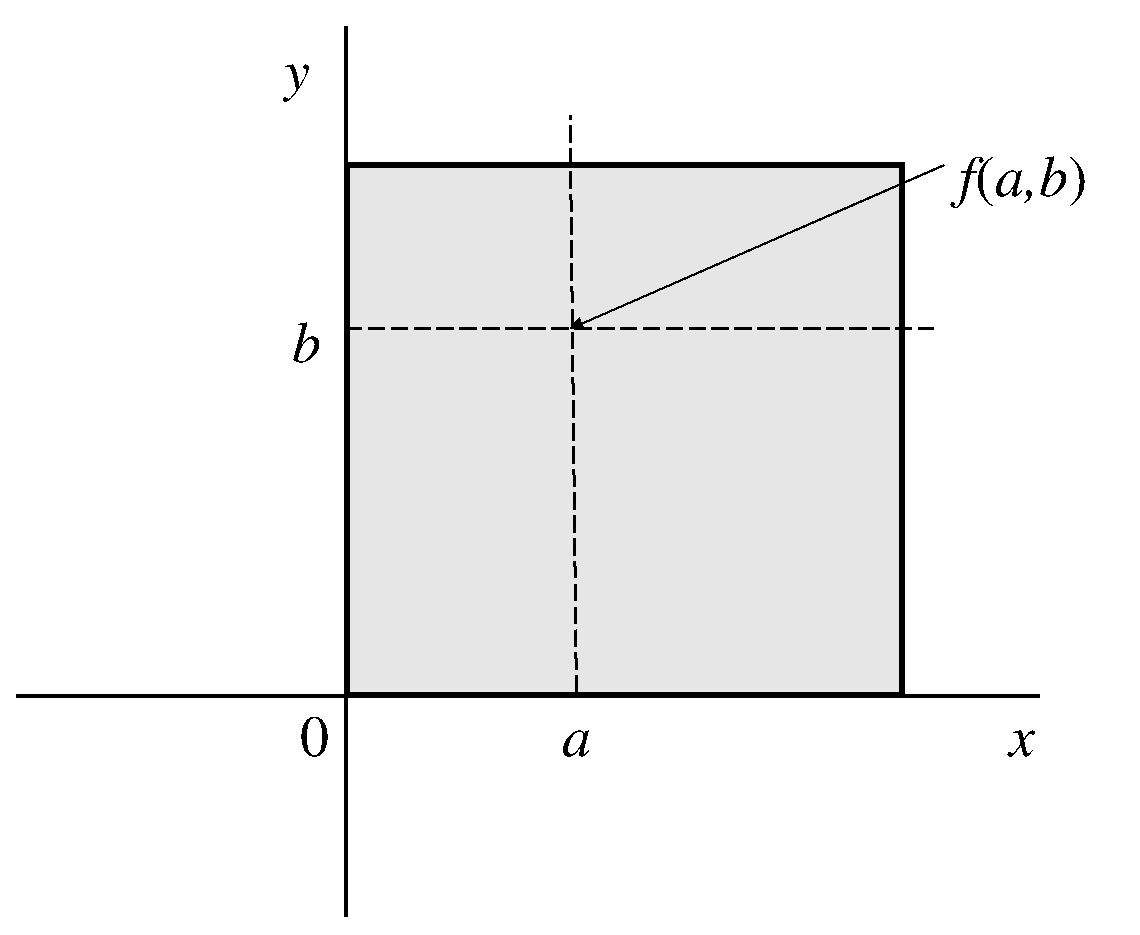
\includegraphics[width=.98\textwidth]{fig/zu-7-2-b.eps}

(b) 2次元信号
\end{center}
\end{minipage}\\[.3\baselineskip]
\begin{minipage}{.35\textwidth}
\begin{center}
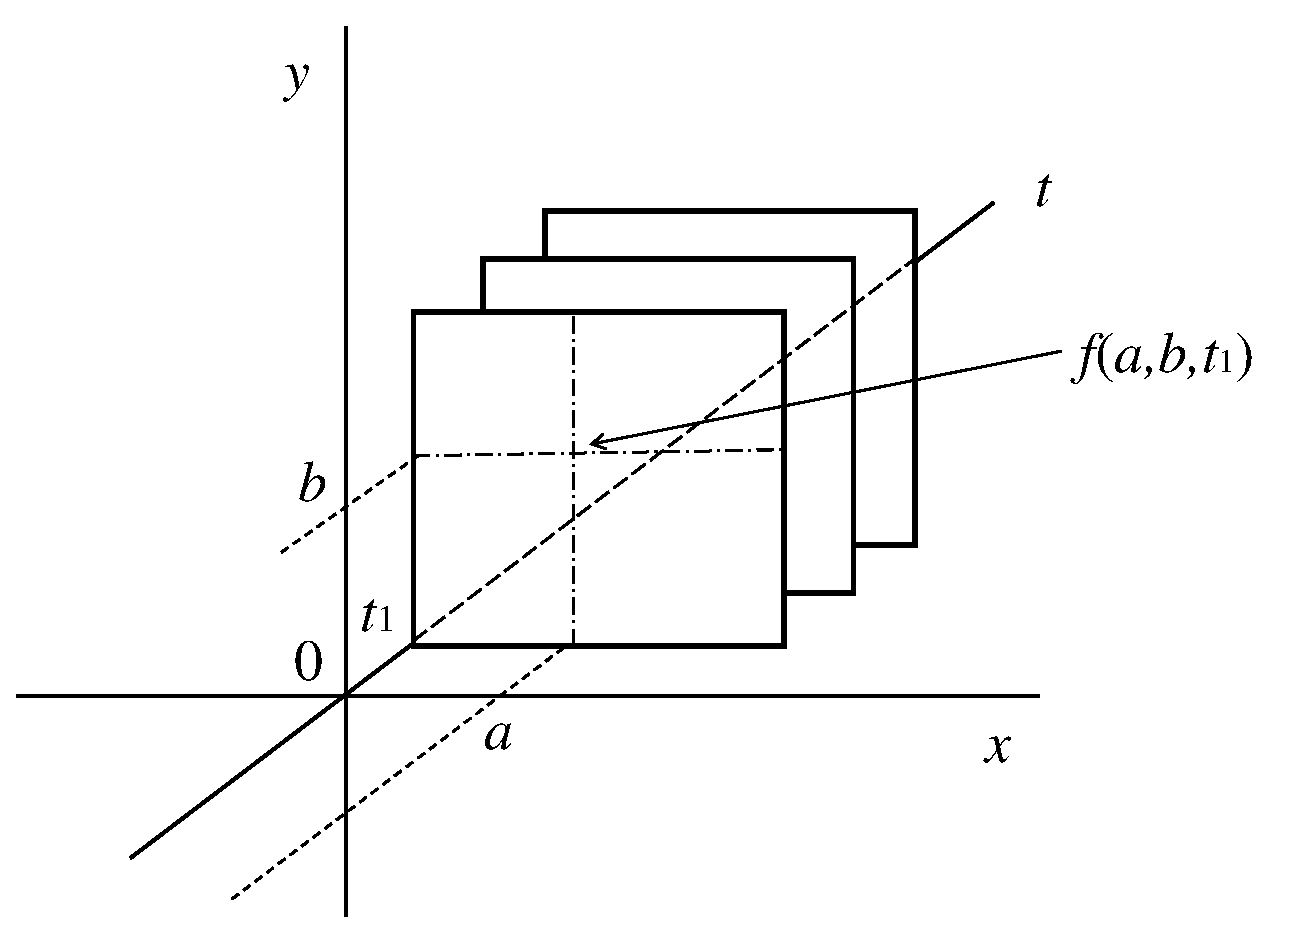
\includegraphics[width=.98\textwidth]{fig/zu-7-2-c.eps}

(c) 3次元信号
\end{center}
\end{minipage}
\end{center}\vskip.3\baselineskip
\caption{信号の次元}
\label{fig:zu-07-2}
\end{figure}

動画像のような3次元信号は,場所$x,y$だけでなく時間$t$も関数に加わったもので,関数$f(x,y,t)$として表される.フレームと呼ばれる多数の2次元信号を時間的に切り替えて表現する.なお,3次元画像もしくは立体画像と呼ばれるものは,場所に関する3次元$x,y,z$を考えたものである.


\subsubsection{サンプリングと量子化}

ディジタル画像信号は,その基となるアナログ信号を\index{さんぷりんぐ@サンプリング}サンプリングし,さらに\index{りょうしか@量子化}量子化することで生成される.

静止画像を例にとると,場所$x,y$についてサンプリングすることで,\index{がそ@画素}画素(pixel)と呼ばれる点の集まりとし,各画素における関数の値を量子化することでディジタル画像が表現される.
%
縦と横との画素数をそれぞれ示すことにより,ディジタル画像のサイズを表すことがあり,その画素数を\index{かいぞうど@解像度}解像度ともいう.たとえば,4Kと呼ばれるディスプレイのサイズは3840$\times$2160である\footnote{テレビ放送やテレビ受像機などのような4K UHDでは384$\times$2160画素であるが,映画やカメラで用いられるDCI 4Kは4096$\times$2160であり,いずれにしても横方向の画素数は4K=4000前後の値であるため,そのような呼び方となっている.なおKはSI接頭語のキロである.}.

サンプリングされた各画素は量子化され,有限なビット数の値で表現される.濃淡画像であれば8bit(256階調)で表されることが多く,プリンタなどで表示するために1bit(白黒2階調)で表現することもある.

カラー画像であれば,赤(Red),緑(Green),青(Blue)の3原色(RGB)を用いて表現することができることから,カラー画像はR,G,Bの信号に対応する3枚の画像に分離される.この分離されたR,G,Bに関する3枚の各画像の画素がそれぞれ8bitに量子化されている場合,その画像をフルカラー画像という\footnote{カラー画像の表現において必ずしもRGBの3原色である必要はなく,目的に応じてYIQや$YC_bC_r$などで表現することもある.}.

\section{画像処理:階調濃度の変換}

ここでは,濃淡画像に対する階調濃度の変換として,明るさの増加,明るさの減少,ネガポジ変換について示す.

階調数削減とは,プリンタで印刷を行う際に,プリンタが持ち合わせている色(シアン:C,マゼンタ:M,イエロー:Y)で印刷可能となるようにフルカラー画像(一般的に1677万色といわれる)を8色にする処理である.また,濃淡画像(白から黒まで256階調の画像)の場合であれば白と黒の2階調に削減する処理である.


\begin{figure}[b]
\begin{center}
\begin{minipage}{.38\textwidth}
\begin{center}

\includegraphics[width=.98\textwidth]{fig/hair1.eps}

(a) 原画像
\end{center}
\end{minipage}
\begin{minipage}{.38\textwidth}
\begin{center}

\includegraphics[width=.98\textwidth]{fig/hair1_p50.eps}

(b) 明るさを増加 ($+50$)
\end{center}
\end{minipage}\\[.5\baselineskip]
\begin{minipage}{.38\textwidth}
\begin{center}

\includegraphics[width=.98\textwidth]{fig/hair1_m50.eps}

(c) 明るさを増加 ($-50$)
\end{center}
\end{minipage}
\begin{minipage}{.38\textwidth}
\begin{center}
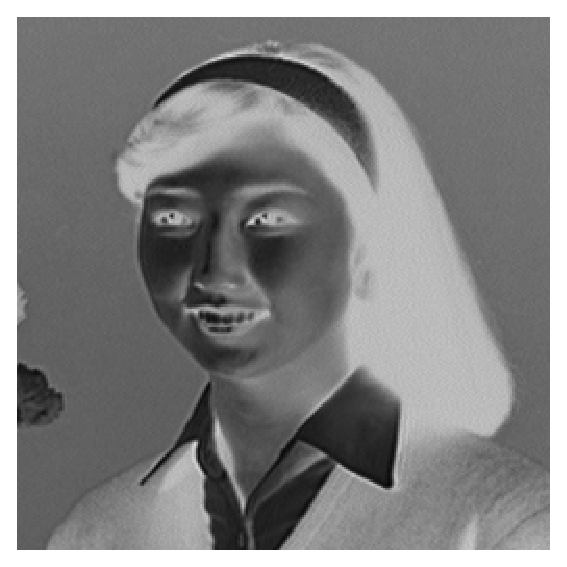
\includegraphics[width=.98\textwidth]{fig/hair1_np.eps}

(d) ネガポジ変換
\end{center}
\end{minipage}
\end{center}\vskip.5\baselineskip
\caption{画像の階調濃度変換}
\label{fig:008-05}
\end{figure}

図\ref{fig:008-05}(a)は256階調の濃淡画像であり,映像情報メディア学会の``ITE標準絵柄-ヘアーバンドの女性''ある.この濃淡画像においては各画素$0\sim 255$の値をとり,黒が0である.


図\ref{fig:008-05}(b)は各画素の値に50を加えたものであり,255を超える場合は255にしている.
\begin{equation}
g(x,y)=
\left \{
\begin{array}{cc}
255 & (f(x,y)+50\geq 255) \\
f(x,y)+50 & \textrm{(otherwize)}
\end{array}
\right .
\end{equation}
この場合は原画像と比較すると明るい画像となっている.

図\ref{fig:008-05}(c)は各画素の値から50を減じたものであり,負数になった場合でも0にしている.
\begin{equation}
g(x,y)=
\left \{
\begin{array}{cc}
0 & (f(x,y)-50\leq 0) \\
f(x,y)-50 & \textrm{(otherwize)} \\
\end{array}
\right .
\end{equation}
この場合は原画像と比較すると暗い画像となっている.

図\ref{fig:008-05}(d)は255から各画素の値を減じたものである.
\begin{equation}
g(x,y)=255-f(x,y)
\end{equation}
原画像において白い部分が黒く表現され,原画像において黒い部分が白く表現されており,白黒が反転していることがわかる.このことからネガポジ変換と呼ばれることがある.
なお,このような階調濃度の変換にはこれ以外にもさまざまな方法があり,所望の画質が得られるような変換を用いることが重要である.



\section{画像処理:画像の2値化}

%ここでは,プリンタに表示するための画像処理である画像の2値化について説明する.

たとえば,プリンタに画像を印刷させる際には,カラー印刷の場合,\index{しあん@シアン}シアン(C),\index{まぜんた@マゼンタ}マゼンタ(M),\index{いえろー@イエロー}イエロー(Y),\index{すみ@墨}墨(K)なる4色のインクもしくはトナーによって表現するため,これらの色が表示される点の密度を調節することによって,原画像の色に近い表現となるようにしている.そのための画像処理として,画像の2値化について説明する.ここでは,簡単のため,白と黒だけで構成された画像(白黒2値画像)にする.

濃淡画像は256階調(0~255の整数)となっている.
%
図\ref{fig:008-06}(b)は各画素における階調濃度が127以下であれば0,128以上であれば255となるように2値化したものである.つまり,
\begin{equation}
g(x,y)=
\left \{
\begin{array}{cc}
255 & (f(x,y)\geq 128) \\
0 & (それ以外)
\end{array}
\right .
\end{equation}
の処理を行ったものである.これだと白と黒の中間的な部分をうまく表現できていないことがわかる.

図\ref{fig:008-06}(c)は\index{でぃざほう@ディザ法}ディザ法により2値化した画像である.これは画像を4$\times$4画素のブロックに分割して,そのブロック内において図\ref{fig:dither_m}で示されるディザ行列のように閾値を変化させたものである.これは,見かけ上,原画像に周期的な雑音を重畳させて2値化したものと見なすことができるため,白と黒との中間的な部分による表現が改善され,グレーに見えるようになっている.しかしながら,このディザ法による2値画像だと輪郭の部分がぼけて見えるという問題などがある.

\begin{figure}[H]
\begin{center}
\begin{tabular}{|c|c|c|c|}
\hline
0 & 8 & 2 & 10 \\
\hline 
12 & 4 & 14 & 6 \\
\hline
3 & 11 & 1 & 9 \\
\hline
15 & 7 & 13 & 5 \\
\hline 
\end{tabular}
\end{center}
\caption{ディザ行列}
\label{fig:dither_m}
\end{figure}

図\ref{fig:008-06}(d)は\index{ごさかくさんほう@誤差拡散法}誤差拡散法と呼ばれる2値化の手法を用いたものである.これは,2値化をする際に発生した誤差$\Delta(x,y)=f(x,y)-g(x,y)$を量子化されていない画素へ繰り込む方式である.この処理を行うことで輪郭の部分がより明確に表現され,白と黒との中間的な部分におけるノイズのように感じられる現象も緩和されていることがわかる.

\begin{figure}[H]
\begin{center}
\begin{minipage}{.38\textwidth}
\begin{center}

\includegraphics[width=.98\textwidth]{fig/hair1.eps}

(a) 原画像
\end{center}
\end{minipage}
\begin{minipage}{.38\textwidth}
\begin{center}
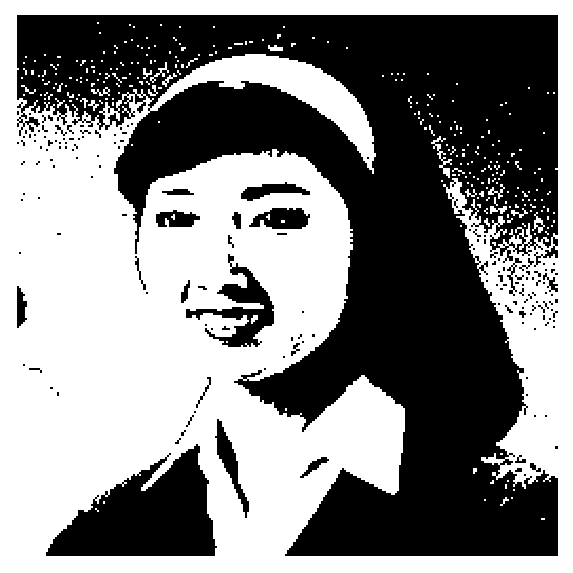
\includegraphics[width=.98\textwidth]{fig/hair1_bin.eps}

(b) 閾値(127)で白黒2値化
\end{center}
\end{minipage}\\[.5\baselineskip]
\begin{minipage}{.38\textwidth}
\begin{center}
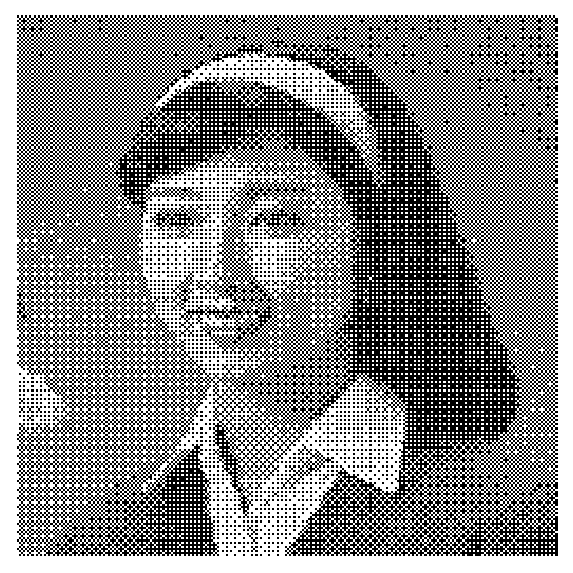
\includegraphics[width=.98\textwidth]{fig/hair1_dither.eps}

(c) ディザ法を用いた2値化
\end{center}
\end{minipage}
\begin{minipage}{.38\textwidth}
\begin{center}
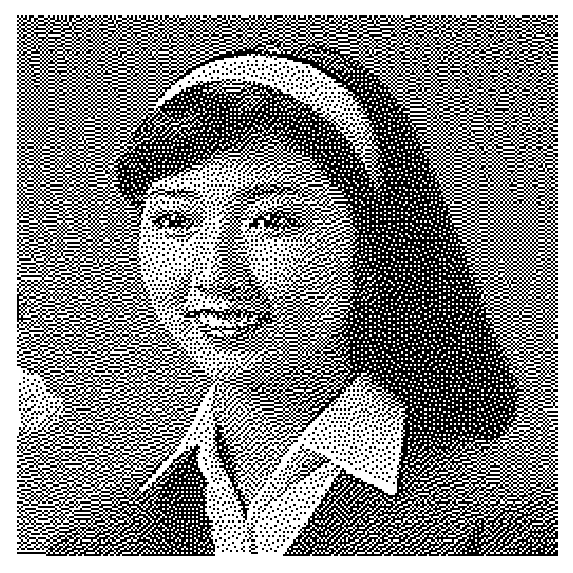
\includegraphics[width=.98\textwidth]{fig/hair1_ed.eps}

(d) 誤差拡散法による2値化
\end{center}
\end{minipage}
\end{center}\vskip.5\baselineskip
\caption{画像の2値化処理}
\label{fig:008-06}
\end{figure}

\section{画像のフィルタ処理}

ここでは画像に対してフィルタ処理を行った例について述べる.フィルタ処理には,ぼかし,尖鋭化などの処理がある.
%
図\ref{fig:008-07}は画像の処理として,ぼかしや尖鋭化などに関する結果を示している.ここで原画像は図\ref{fig:008-05}(a)である.

\begin{figure}[H]
\begin{center}
\begin{minipage}{.38\textwidth}
\begin{center}

\includegraphics[width=.98\textwidth]{fig/hair1_bokashi.eps}

(a) ぼかし
\end{center}
\end{minipage}
\begin{minipage}{.38\textwidth}
\begin{center}
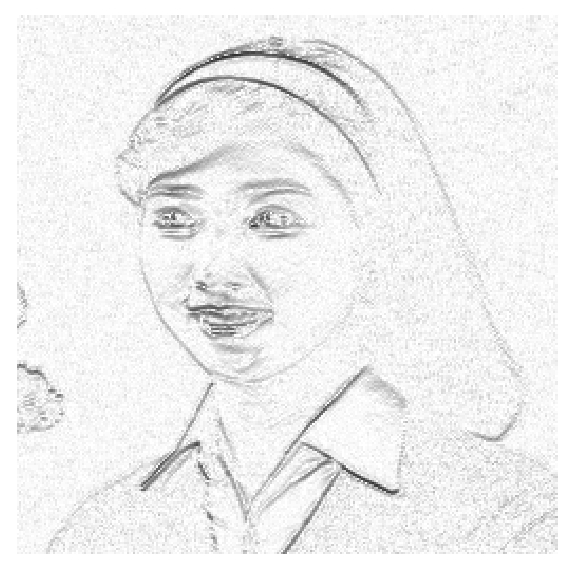
\includegraphics[width=.98\textwidth]{fig/hair1_x_sharp.eps}

(b) x軸方向に関する階調濃度の変化
\end{center}
\end{minipage}\\[.5\baselineskip]
\begin{minipage}{.38\textwidth}
\begin{center}
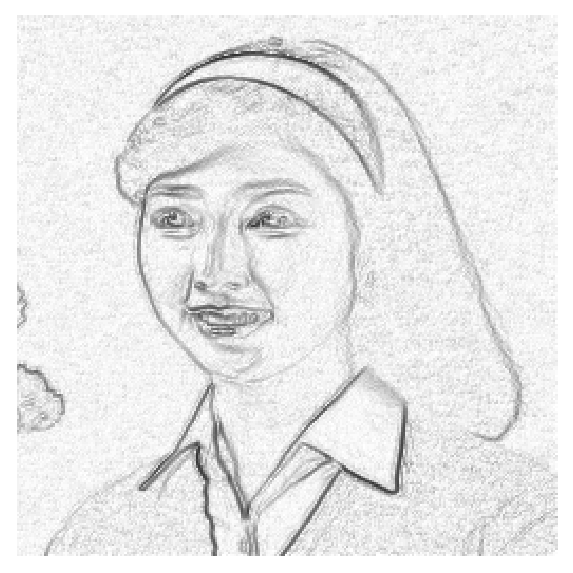
\includegraphics[width=.98\textwidth]{fig/hair1_rinkaku.eps}

(c) 輪郭流出
\end{center}
\end{minipage}
\begin{minipage}{.38\textwidth}
\begin{center}

\includegraphics[width=.98\textwidth]{fig/hair1_sharp.eps}

(d) 輪郭の尖鋭化
\end{center}
\end{minipage}
\end{center}\vskip.5\baselineskip
\caption{画像処理の例(原画像は図\ref{fig:008-05}(a))}
\label{fig:008-07}
\end{figure}



図\ref{fig:008-07}(a)は画像のぼかしをした例である.これはしわの除去などを目的とした処理の原理となるものである.
\begin{equation}
g(x,y)=\sum_{i=-1}^{1} \sum_{j=-1}^{1} f(x+i,y+j)t(i,j)
\end{equation}
と表現され,フィルタ行列である$t(i,j)$は
\begin{equation}
t(i,j)=\frac{1}{9} \left (
\begin{array}{ccc}
1 & 1 & 1 \\
1 & 1 & 1 \\
1 & 1 & 1 \\
\end{array}
\right )
\end{equation}
としている.このぼかし処理は周辺画素との平均値を求めることによる方法であるが,このフィルタ行列の要素数や値を変化させることで,ぼかしの度合いを変化させることもできる.


図\ref{fig:008-07}(b)は画像のx軸方向における階調濃度変化がある部分を黒くなるようにしたものである.
\begin{equation}
g(x,y)=255-|f(x,y)-f(x+1,y)|
\end{equation}
輪郭となる部分は階調濃度が大きく変化するので,階調濃度に関する微分をとればよいように思われるが,これでは十分な輪郭抽出がなされてるとはいえない.

図\ref{fig:008-07}(c)は画像のラプラシアン(x軸方向およびy軸方向における2階偏微分)をとったものである.

\begin{eqnarray}
g(x,y)&=& \nabla^2 f(x,y) \nonumber \\
 &=&\sum_{i=-1}^{1} \sum_{j=-1}^{1} f(x+i,y+j)t(i,j)
\end{eqnarray}\vskip.3\baselineskip

\noindent と表現され,フィルタ行列である$t(i,j)$は
\begin{equation}
t(i,j)=\left (
\begin{array}{ccc}
0 & 1 & 0 \\
1 & -4 & 1 \\
0 & 1 & 0 \\
\end{array}
\right )
\end{equation}
である.この場合だと,\index{りんかくちゅうしゅつ@輪郭抽出}輪郭抽出がなされているといえる.この処理をベースとした輪郭線抽出の後,\index{ぱたーんにんしき@パターン認識}パターン認識を行うという場合もある.

図\ref{fig:008-07}(d)は図\ref{fig:008-05}(a)の輪郭をシャープに見えるように処理したものである.これは図\ref{fig:008-05}(a)に図\ref{fig:008-07}(c)をあわせたものとみることができる.

このような輪郭抽出は,ぼけた画像から輪郭の部分を明瞭にするためであったり,塗り絵のための画像を生成したりするために有効とされる.またぼかしはしみやしわを除去したり,ある一定の情報が特定されないようにしたりするための処理などで用いられる.

\section*{演習問題}

\subsection*{問題\ref{chapter:image}.1}

次のような$4\times 4$画素で8bitのデータが図\ref{fig:ima-d}のようにある.
以下の問に答えよ.
\begin{enumerate}[(1)]
\item 図\ref{fig:ima-d}における\index{ひすとぐらむ@ヒストグラム}ヒストグラムを示せ.
\item 図\ref{fig:ima-d}のネガポジ画像はどのようなデータになるか示せ.
\item 図\ref{fig:dither_m}に示すディザ行列を用いる場合,図\ref{fig:ima-d}がディザ法を掛けた場合にどのような結果となるか示せ.ただし,図\ref{fig:dither_m}のディザ行列は4bitでできていることに注意せよ.
\end{enumerate}

\begin{figure}[H]
\begin{center}
\begin{tabular}{|c|c|c|c|}
\hline
20 & 90 & 165 & 250 \\
\hline 
20 & 90 & 165 & 250 \\
\hline
20 & 90 & 165 & 250 \\
\hline
20 & 90 & 165 & 250 \\
\hline 
\end{tabular}
\end{center}
\caption{問題\ref{chapter:image}.1のデータ}
\label{fig:ima-d}
\end{figure}





